 %\documentclass{egpublplain}
%\usepackage{egsgp11}
\documentclass[twoside]{article}
%\usepackage[reviewing]{aag10} % for the final version
\usepackage[final]{aag10} % for the final version
\usepackage{subfiles}
\usepackage{color}
\usepackage{url}
\usepackage{contour}
\contournumber{32}
\contourlength{0.1em}
\usepackage{ifsym}
\usepackage[multiple]{footmisc}
\usepackage{amsmath}
\usepackage{amssymb}
\usepackage{url}
\usepackage{paralist}
\usepackage{xspace}
\newcommand{\Epl}{E_{pl}}
\newcommand{\Ereg}{E_{reg}}
\newcommand{\R}{\mathbb{R}}
\newcommand{\VaryLab}{{\sc VaryLab}\xspace}
\newcommand{\nurbs}{{\sc nurbs}\xspace}


% for including postscript figures
% mind: package option 'draft' will replace PS figure by a filname within a frame
\ifpdf \usepackage[pdftex]{graphicx} \pdfcompresslevel=9
\else \usepackage[dvips]{graphicx} \fi

\usepackage[percent]{overpic}
% TODO: remove package import
%\usepackage{showlabels}
%\renewcommand{\showlabelfont}{\scriptsize\ttfamily\color{blue}}
% \PrintedOrElectronic

% prepare for electronic version of your document
% \usepackage{t1enc,dfadobe}

%\usepackage{egweblnk}
\usepackage{cite}

% ams packages
% \usepackage{amssymb}
% \newtheorem{definition}{Definition}[section]

\usepackage{graphicx}
\graphicspath{{images/}}

% For backwards compatibility to old LaTeX type font selection.
% Uncomment if your document adheres to LaTeX2e recommendations.
% \let\rm=\rmfamily    \let\sf=\sffamily    \let\tt=\ttfamily
% \let\it=\itshape     \let\sl=\slshape     \let\sc=\scshape \let\bf=\bfseries
% end of prologue


% ------------------------------------------------------------------------

% if the Editors-in-Chief have given you the data, you may uncomment
% the following five lines and insert it here
%
% \volume{27}   % the volume in which the issue will be published;
% \issue{1}     % the issue number of the publication
% \pStartPage{1}      % set starting page


\newtheorem{definition}{Definition}

%-------------------------------------------------------------------------
\def\mainbibliography {
	\bibliographystyle{acmsiggraph1} % use ACM SIGGRAPH bibliography style
	\bibliography{article}
}
\def\subfilebibliography {
	\bibliographystyle{acmsiggraph1} % use ACM SIGGRAPH bibliography style
	\bibliography{article}
}

\begin{document}
\def\subfilebibliography{}
\title{Surface panelization using periodic conformal maps}
\def\shortauthor{T.~R\"orig, S.~Sechelmann, A.~Kycia, M.~Fleischmann}
\def\shorttitle{Periodic conformal maps}
\author{Thilo R\"orig, Stefan Sechelmann\affiliation{Institut f\"ur Mathematik, Technische Universit\"at Berlin}
Agata Kycia, Moritz Fleischmann\affiliation{HENN Research, HENN Architekten}
}
\maketitle

\begin{abstract}
  We present a new method to obtain periodic conformal
  parameterizations of surfaces with cylinder topology and describe
  applications to architectural design and rationalization of
  surfaces. The method is based on discrete conformal maps from the
  surface mesh to a cylinder or cone of revolution. It accounts for a
  number of degrees of freedom on the boundary that can be used to
  obtain a variety of alternative panelizations. We illustrate
  different choices of parameters for \nurbs surface designs. Further,
  we describe how our parameterization can be used to get a periodic
  boundary aligned hex-mesh on a doubly-curved surface and show the
  potential on an architectural facade case study.  Here we optimize
  an initial mesh in various ways to consist of a limited number of
  planar regular hexagons that panel a given surface.
\end{abstract}
%-------------------------------------------------------------------------

\begin{figure}[h!]
  \centering
  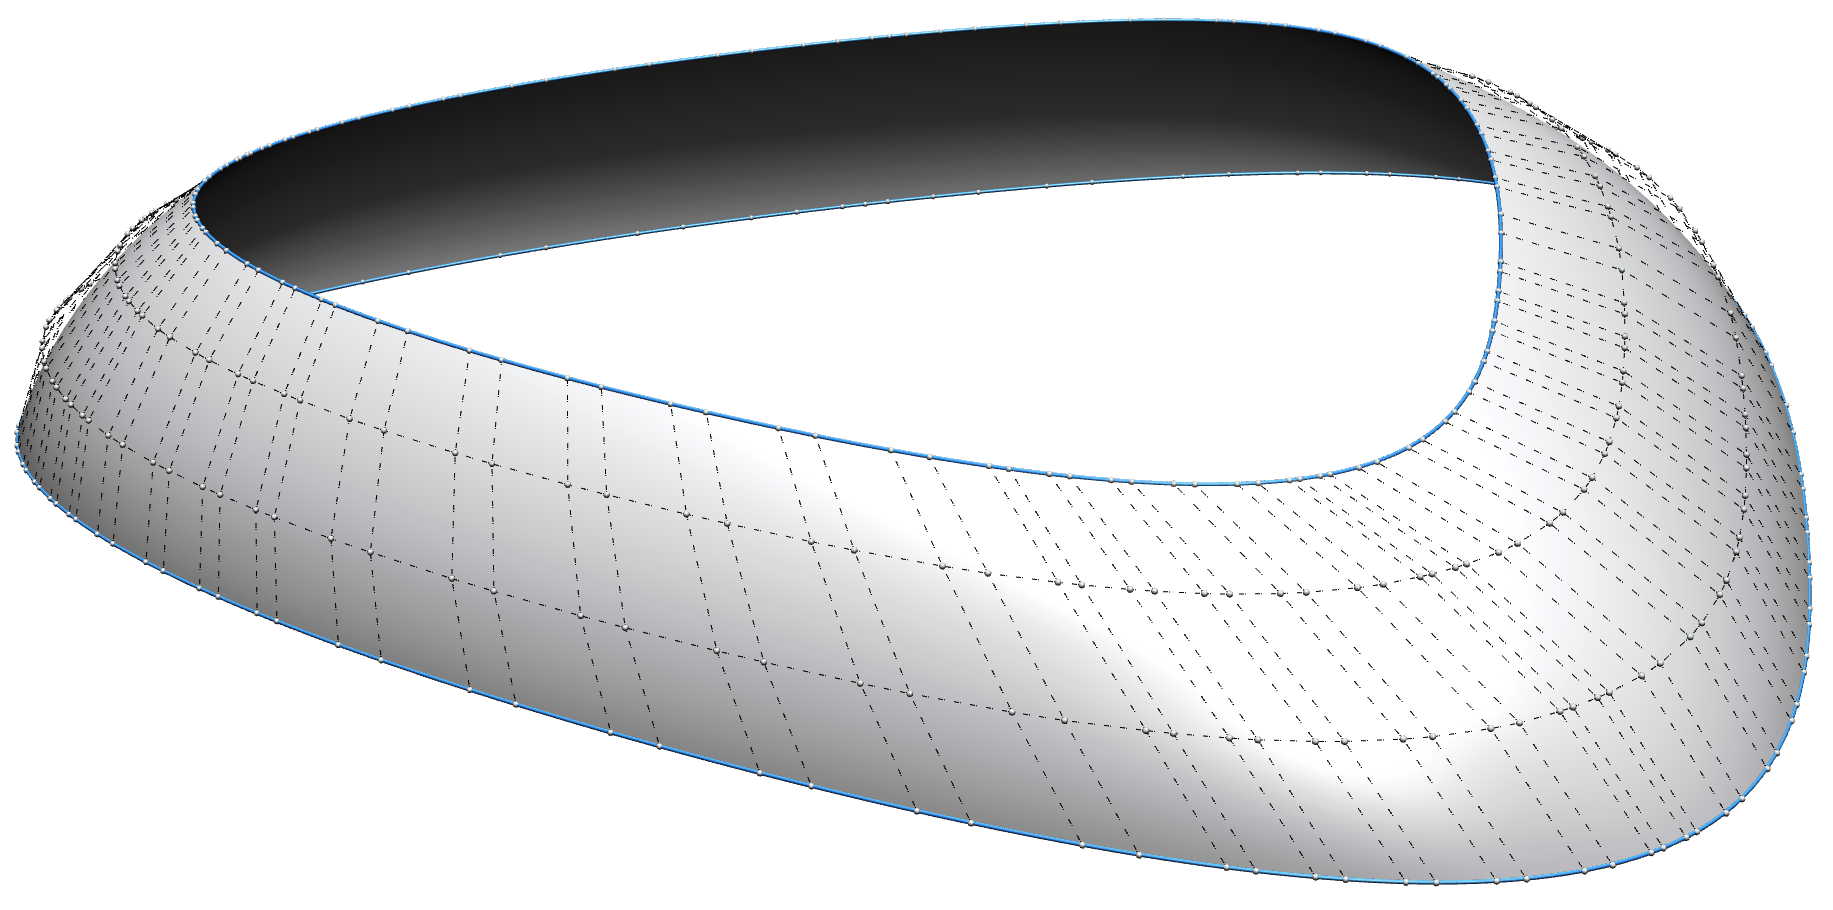
\includegraphics[width=0.49\textwidth]{images/teaser1_grid.png}
  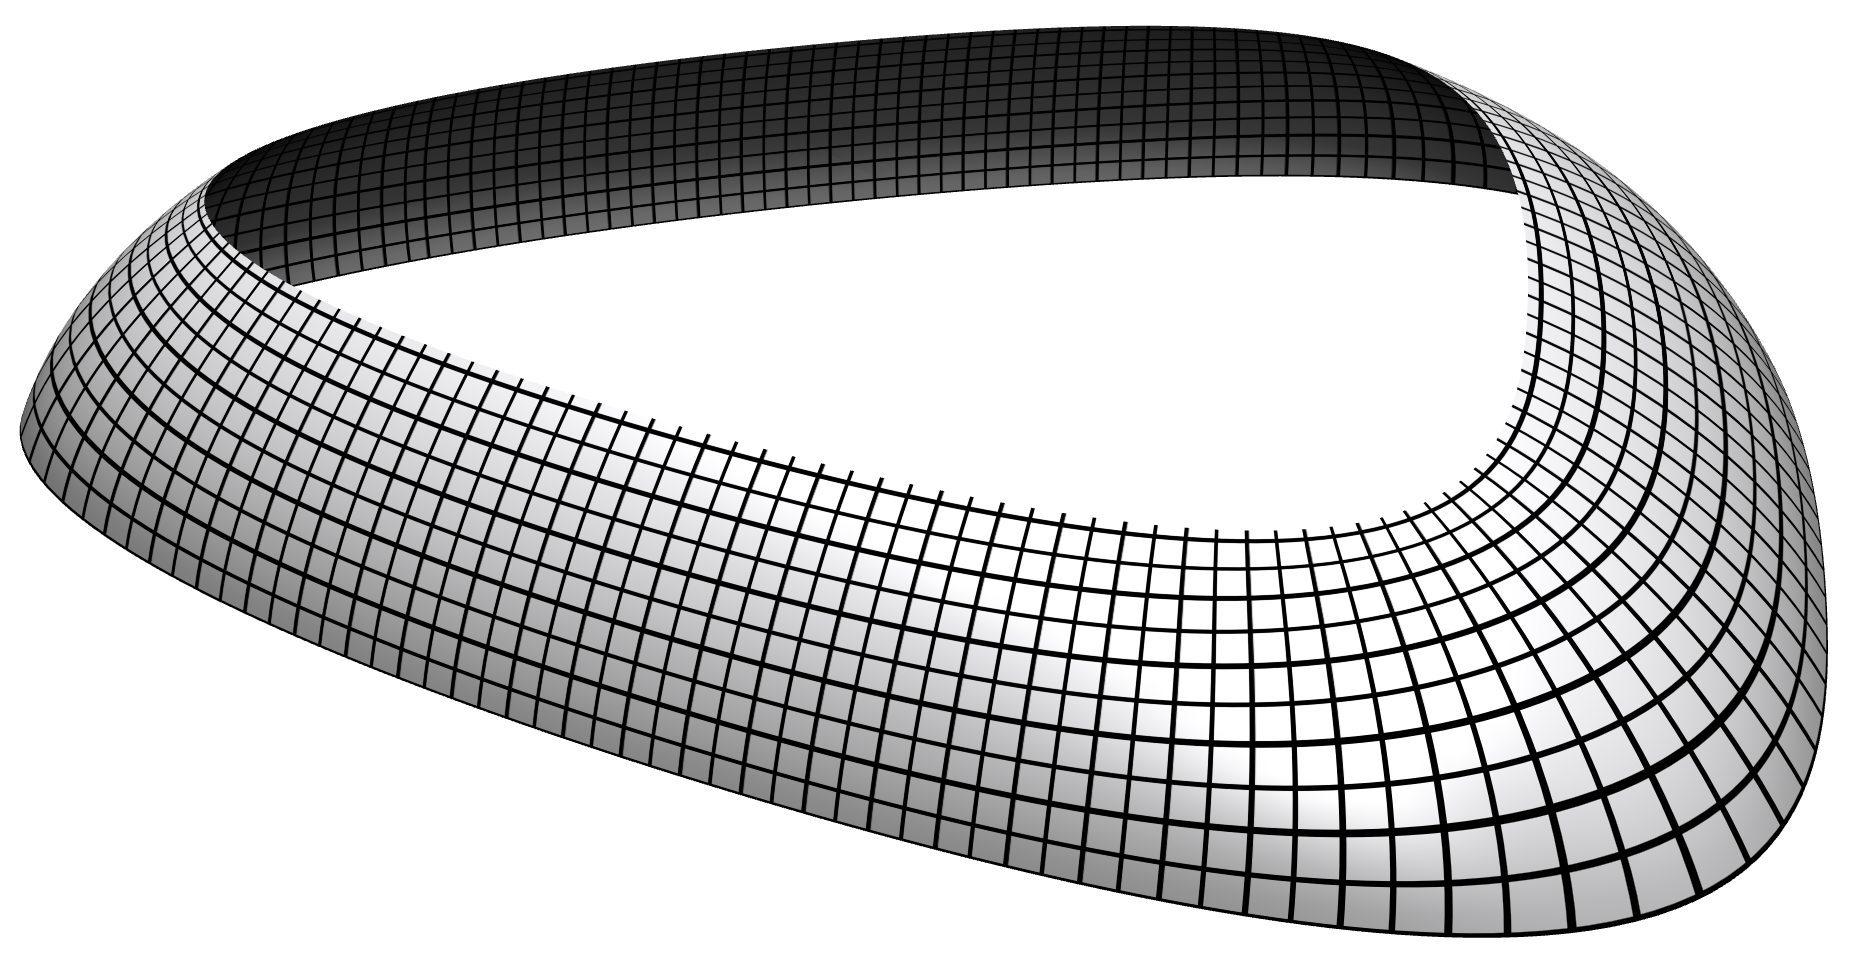
\includegraphics[width=0.49\textwidth]{images/teaser2_2.png}
  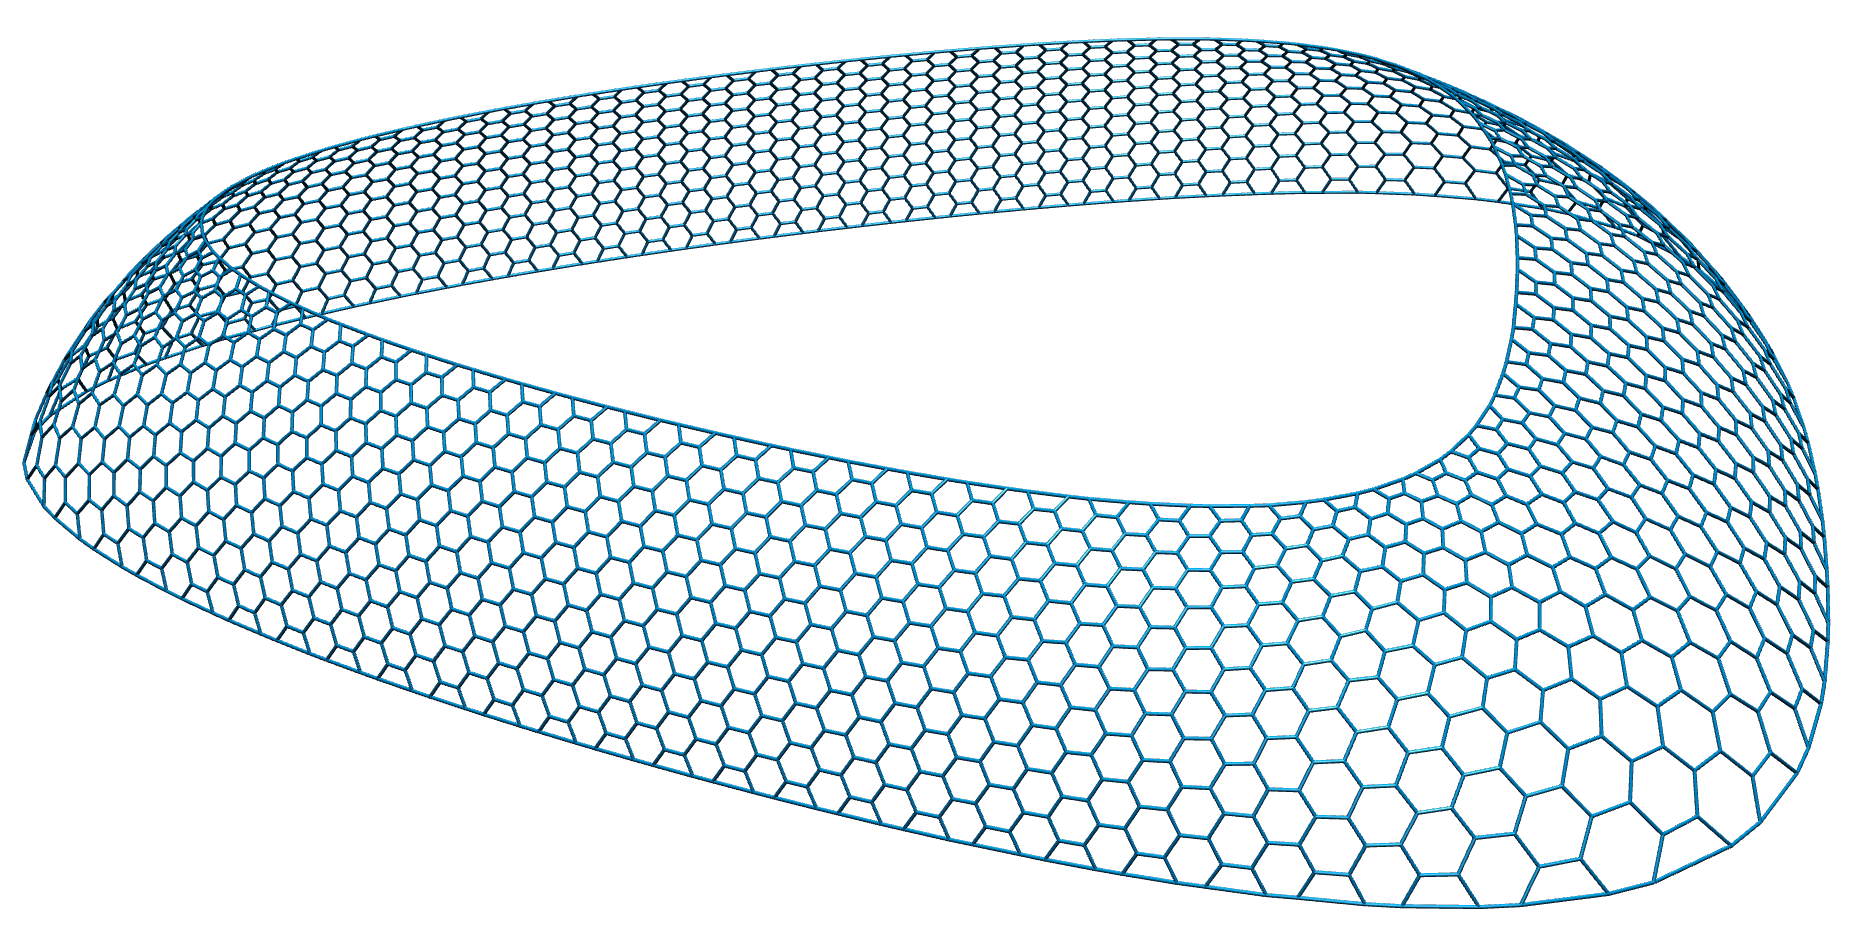
\includegraphics[width=0.49\textwidth]{images/teaser4_1.png}
  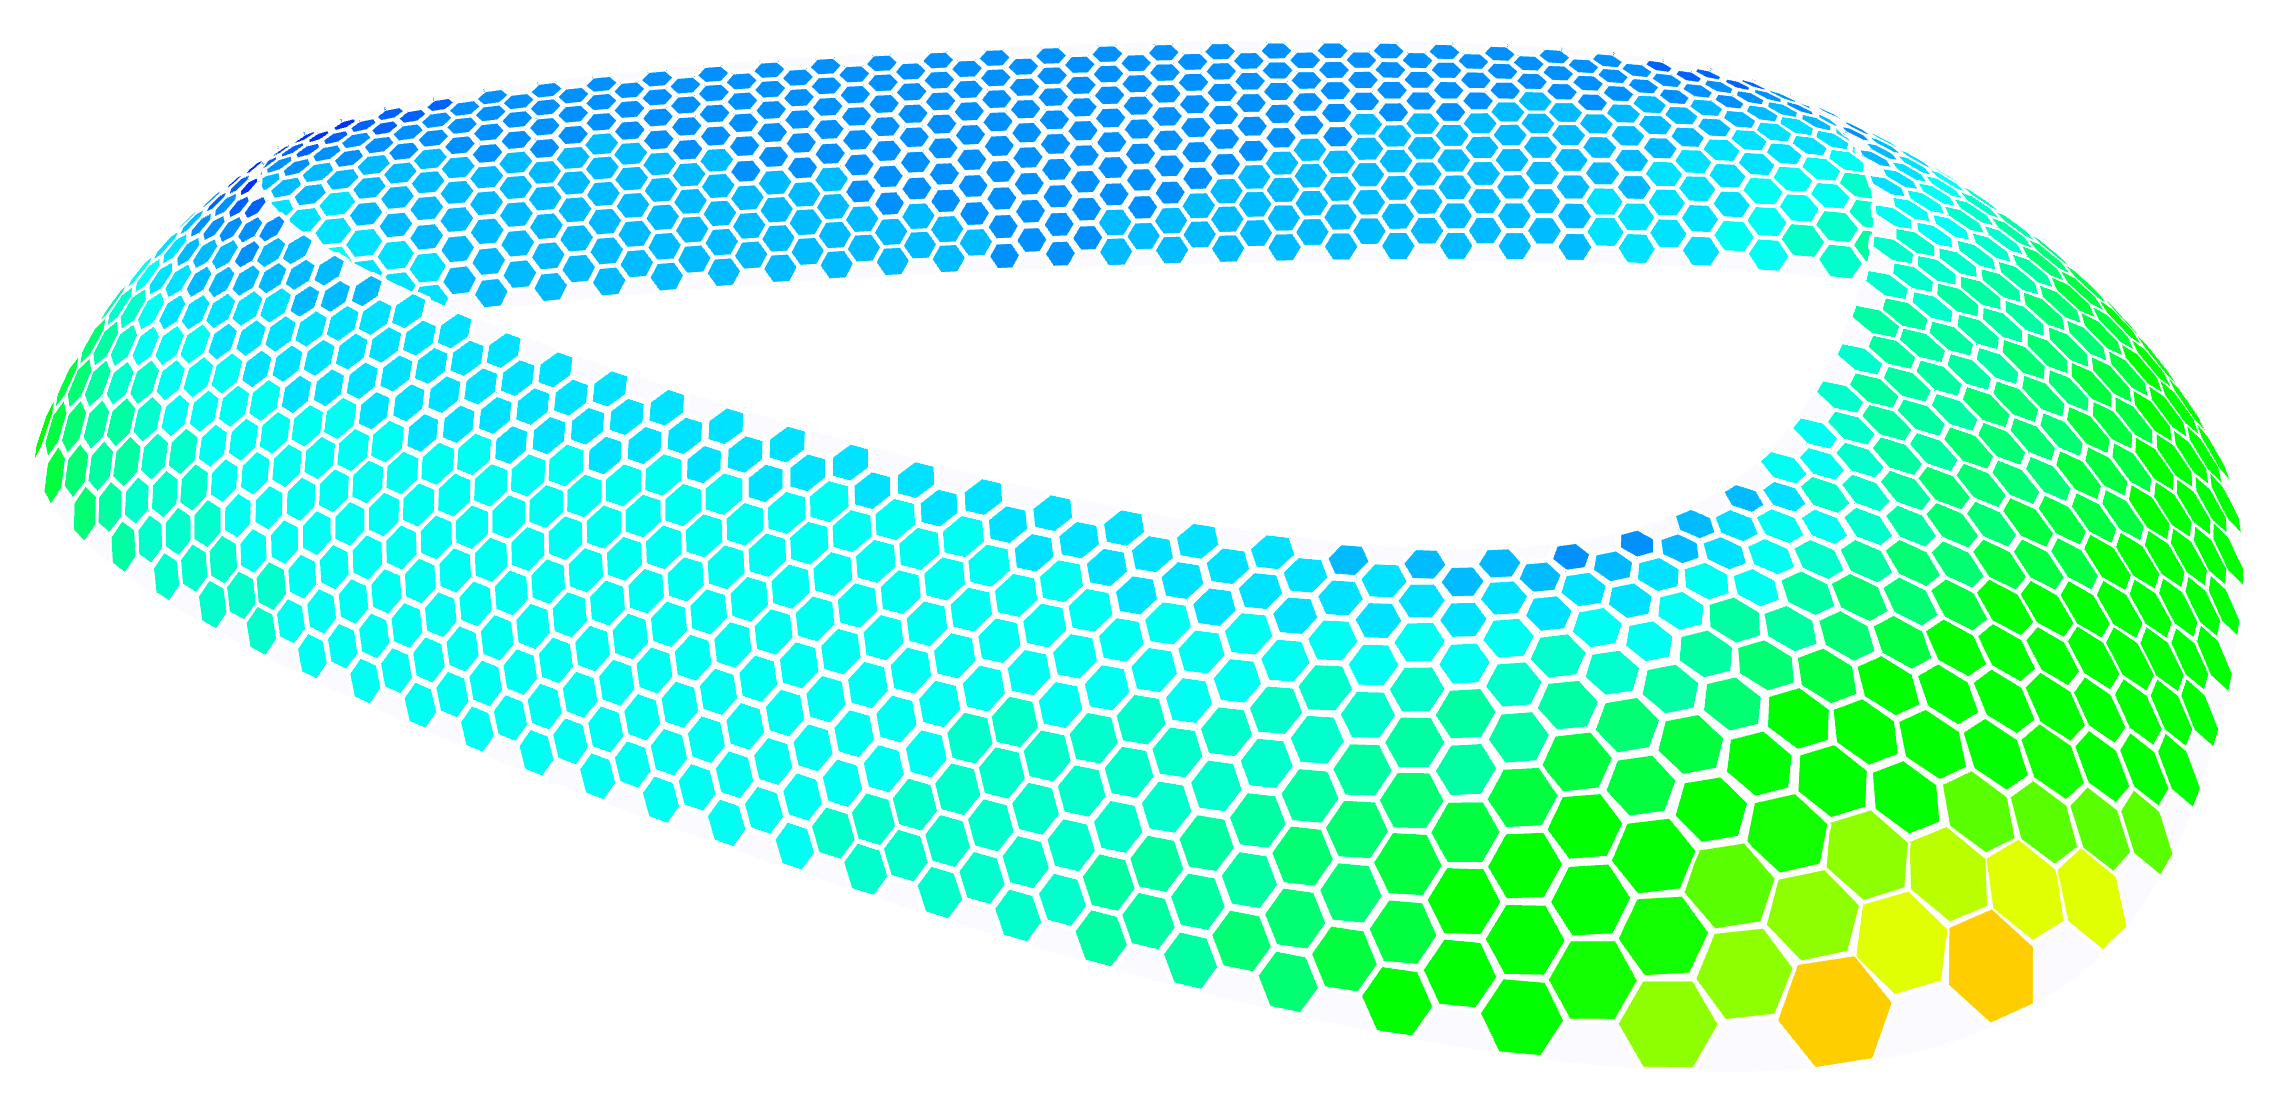
\includegraphics[width=0.49\textwidth]{images/quantized_aligned5.png}
  \caption{Outline of the method: For a cylindrical \nurbs
  surface (top-left) we create a seamless periodic conformal parameterization (top-right). A new
    mesh (bottom-left) is then rationalized and the panels are
    optimized for quantized regular hexagons (bottom-right).}
  \label{fig:teaser}
\end{figure}

\subfile{introduction.tex}
\subfile{parametrization.tex}
\subfile{conformal-parametrization.tex}
\subfile{boundary-conditions.tex}
\subfile{panelization.tex}
\subfile{hexagons.tex}
\subfile{implementation.tex}
\subfile{conclusion.tex}

\section*{Acknowledgements}
We would like to thank Boris Springborn for sharing his knowledge on
discrete conformal maps and the anonymous referees for their comments.
%TODO: Sascha?
Thilo R\"orig and Stefan Sechelmann are supported by SFB/TR 109:
Discretization in Geometry and Dynamics and DFG Research Center
\textsc{Matheon}.


\mainbibliography

\end{document} 
